\chapter{Apartado C: \textbf{Detección de puntos de interés}}
\label{chapter:tarea_c}

En este apartado deberá extraer los puntos de interés de la imagen \texttt{data/partC/0.jpg}. Una vez hecho, podrá comprobar la correspondencia con esa misma imagen girada (\texttt{data/partC/0\_rot.jpg}) y la relación entre ambas (Figura \ref{fig:feat_match}). El código se desarrolla en el notebook \texttt{partC.ipynb}.

\begin{figure}[h]
    \centering
    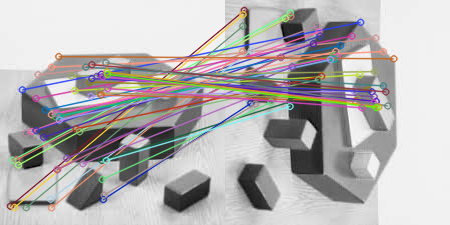
\includegraphics[width=0.6\textwidth]{figures/feature_match_opencv.png}
    \caption{Correspondencia de características entre una imagen y la misma girada, con el SIFT de OpenCV.}
    \label{fig:feat_match}
\end{figure}

A lo largo del apartado se desarrollarán las funciones necesarias para detectar los puntos de interés y calcular sus descriptores empleando la transformación SIFT. La transformación SIFT consta de cuatro pasos principales:

\begin{enumerate}
    \item Detección de extremos en el espacio de escalas.
    \item Localización de los puntos de interés.
    \item Asignación de orientaciones.
    \item Generación de los descriptores de los puntos de interés.
\end{enumerate}

Cada uno se irá desarrollando con las funciones necesarias para completarlo. Se comenzará generando el espacio de escalas en el que se buscarán los extremos.

\section*{Tarea PREVIA: Creación de las carpetas de resultados}
\phantomsection
\addcontentsline{toc}{section}{Tarea PREVIA: Creación de las carpetas de resultados}

Cree la carpeta \texttt{../results/partC} con la subcarpeta \texttt{feature\_extraction}. Dentro de esta última, cree las subcarpetas \texttt{0\_gaussians}, \texttt{1\_difference\_of\_gaussians}, \texttt{2\_match\_features} y \texttt{3\_SIFT}.

\section*{Tarea C.1: Generar función de filtro gaussiano}
\phantomsection
\addcontentsline{toc}{section}{Tarea C.1: Generar función de filtro gaussiano}

Para generar el espacio de escalas que se desea analizar, se debe aplicar un filtrado gaussiano a la imagen original hasta obtener un número de imágenes gaussianas relevante. Para ello, debe desarrollar la función \texttt{generateGaussianImages()} empleando el método \texttt{cv2.GaussianBlur()} \footnote{ \href{https://docs.opencv.org/3.4/d4/d86/group\_\_imgproc\_\_filter.html\#gaabe8c836e97159a9193fb0b11ac52cf1}{Documentación del método \texttt{cv2.GaussianBlur()} en OpenCV:} \\{https://docs.opencv.org/3.4/d4/d86/group\_\_imgproc\_\_filter.html\#gaabe8c836e97159a9193fb0b11ac52cf1}} de la librería OpenCV.

Como entrada, se recibe una imagen y una lista de sigmas que deberá aplicar en el filtrado. Deberá generar tantas imágenes gaussianas como sigmas haya en la lista, aplicando cada filtro al resultado del filtrado anterior (y a la imagen original en el primer caso).

\section*{Tarea C.2: Generación de espacio de escalas con imágenes gaussianas}
\phantomsection
\addcontentsline{toc}{section}{Tarea C.2: Generación de espacio de escalas con imágenes gaussianas}

Deberá cargar la imagen base (\texttt{data/partC/0.jpg}) con cv2 y en escala de grises, sin emplear la función \texttt{cv2.cvtColor()}. A continuación se definen los parámetros iniciales del espacio de escalas: la \textit{sigma} inicial y el número de diferencias de gaussianas que se desea generar (\texttt{intervals}). Aunque el mínimo de diferencias necesarias para detectar los máximos y mínimos en ventanas de 3x3x3 es 3, con ese valor el refinamiento de la localización (Tarea C.5) descarta todos los puntos de interés de esta imagen; por eso el notebook usa \texttt{intervals = 5}. Por último, emplee el método \texttt{generateGaussianImages()} que ha desarrollado en la tarea anterior.

Como puede observar en el código, se le proporciona el método \texttt{generateGaussianSigmas()}, que recibe la \textit{sigma} inicial y el número de diferencias de gaussianas que desea generar. Este método devuelve la lista de valores de \textit{sigma} que deberá aplicar en los filtrados consecutivos: si quiere generar \textit{n} diferencias de gaussianas, le devolverá \textit{n+1} valores de sigma. La Figura \ref{fig:gauss_blur} muestra el resultado esperado de esta tarea.

\begin{figure}[h]
    \centering
    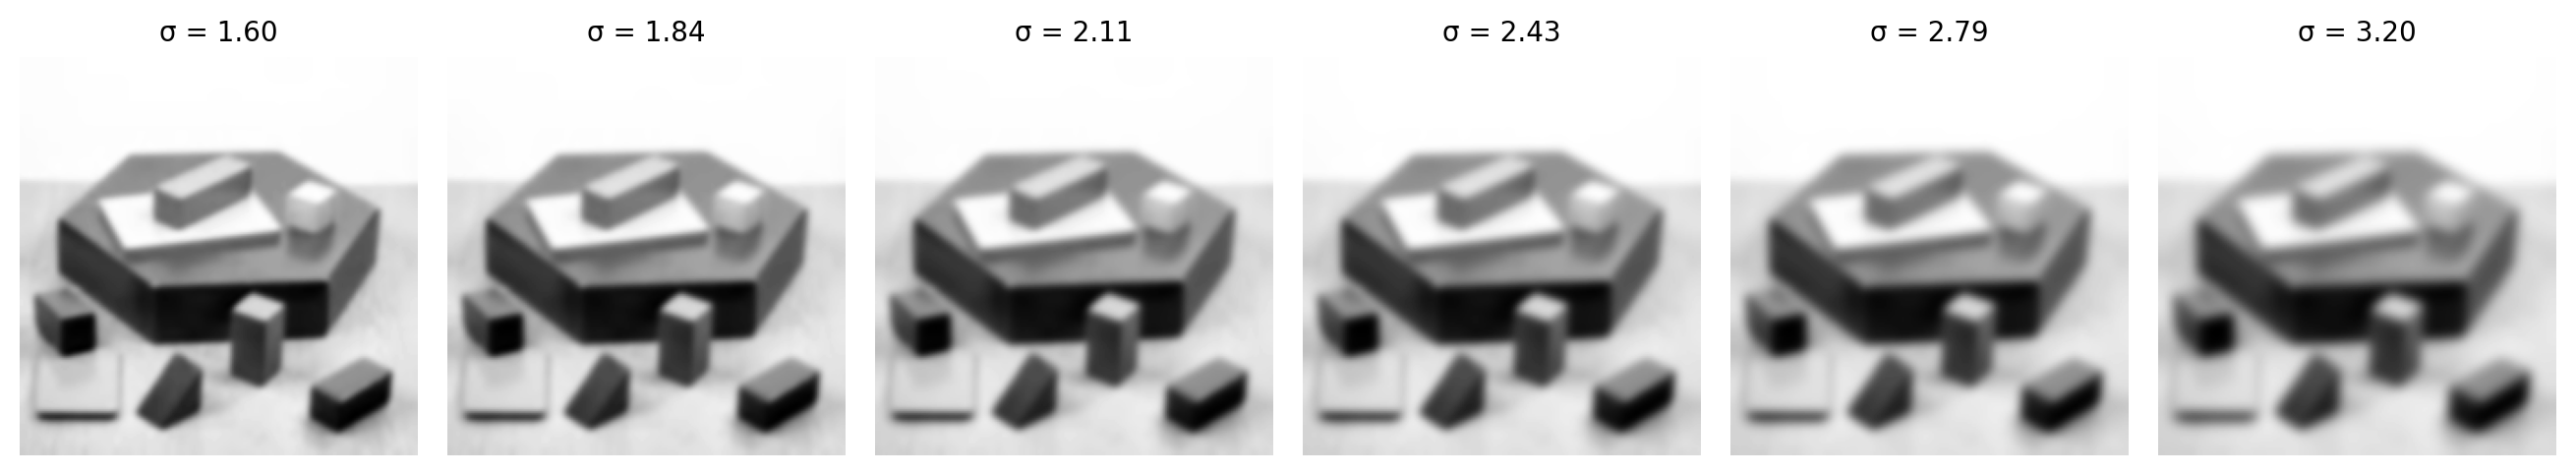
\includegraphics[width=\textwidth]{figures/gaussian_images.png}
    \caption{Resultado esperado de la generación de imágenes gaussianas (\textit{sigma} total acumulada en cada imagen).}
    \label{fig:gauss_blur}
\end{figure}

\section*{Tarea C.3: Generación de diferencias de gaussianas}
\phantomsection
\addcontentsline{toc}{section}{Tarea C.3: Generación de diferencias de gaussianas}

A partir de la lista de imágenes anteriores, se deberá generar una nueva lista con las diferencias entre imágenes consecutivas empleando el método \texttt{cv2.subtract()} \footnote{ \href{https://docs.opencv.org/3.4/d2/de8/group\_\_core\_\_array.html\#gaa0f00d98b4b5edeaeb7b8333b2de353b}{Documentación del método \texttt{cv2.subtract()} en OpenCV:} \\{https://docs.opencv.org/3.4/d2/de8/group\_\_core\_\_array.html\#gaa0f00d98b4b5edeaeb7b8333b2de353b}} de la librería OpenCV. La Figura \ref{fig:dog} muestra el resultado esperado de esta tarea.

\begin{figure}[h]
    \centering
    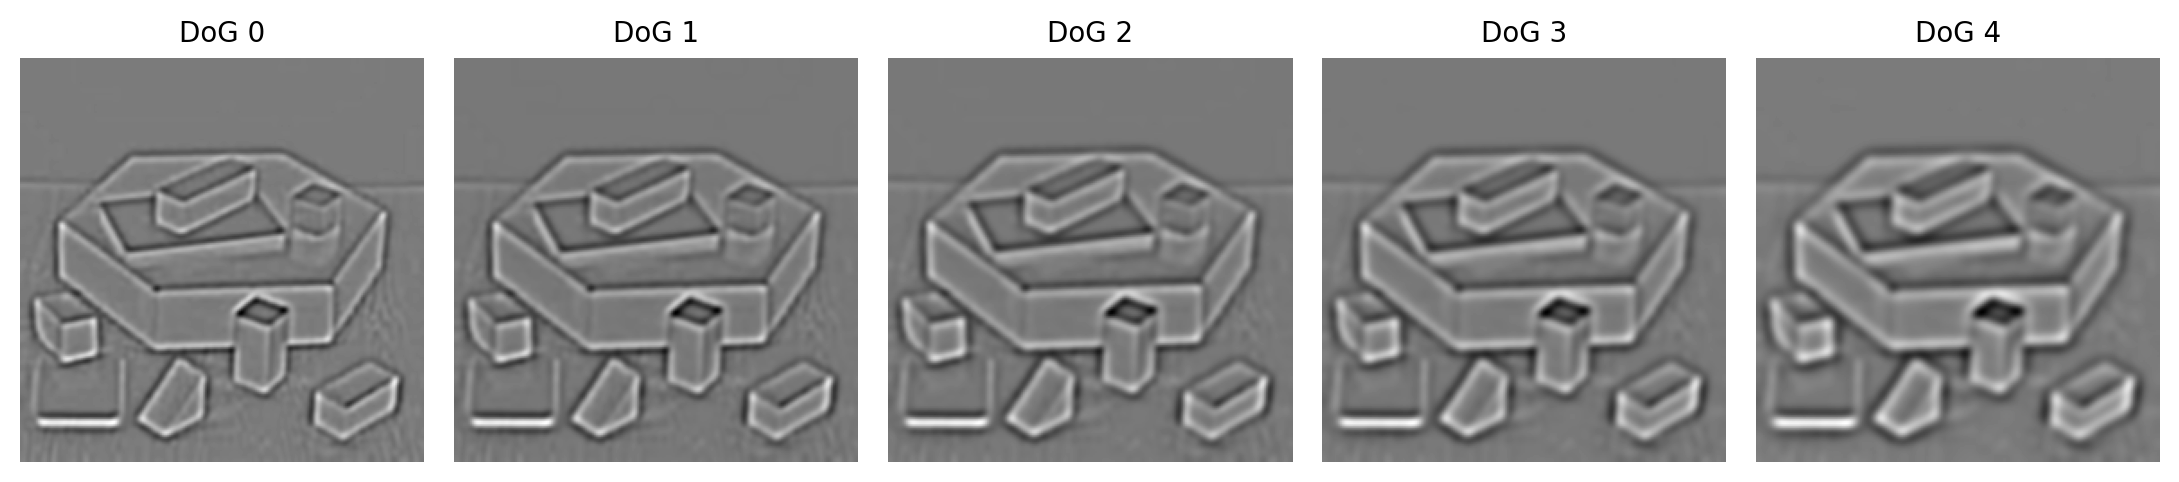
\includegraphics[width=\textwidth]{figures/dog_images.png}
    \caption{Resultado esperado de la generación de diferencias de gaussianas (valores reescalados para su visualización).}
    \label{fig:dog}
\end{figure}

\section*{Tarea C.4: Evaluación de extremos}
\phantomsection
\addcontentsline{toc}{section}{Tarea C.4: Evaluación de extremos}

En esta tarea debe desarrollar la función \texttt{isPixelAnExtremum()}, que evalúa si el píxel central de una ventana de 3x3x3 es un máximo o un mínimo entre sus vecinos y si supera un umbral mínimo en valor absoluto. La ventana está compuesta por 3 regiones de 3x3 píxeles, que corresponden a regiones de 3 diferencias de gaussianas consecutivas. La función debe devolver \textit{True} en caso de ser un máximo o un mínimo y \textit{False} en cualquier otro caso. \textbf{Importante:} las diferencias de gaussianas pueden tomar valores negativos.

\section*{Tarea C.5: Localización de puntos clave y orientación de los mismos}
\phantomsection
\addcontentsline{toc}{section}{Tarea C.5: Localización de puntos clave y orientación de los mismos}

En esta tarea deberá completar la función \texttt{findScaleSpaceExtrema()}, que emplea la función de la tarea anterior.

Primero tendrá que completar el bucle \texttt{for} para obtener en cada iteración 3 diferencias de gaussianas consecutivas y enumerarlas. Tras esto, deberá iterar sobre las coordenadas de la imagen teniendo en cuenta que la ventana de 3x3 debe recorrer toda la imagen sin que ninguno de sus puntos quede fuera de ella. Complete la llamada a la función \texttt{isPixelAnExtremum()} con los argumentos pertinentes para evaluar si el píxel en las coordenadas de esa iteración es un extremo.

Los píxeles que son máximos o mínimos dan una localización aproximada de los puntos de interés de la imagen. La función \texttt{localizeExtremumViaQuadraticFit()} (ya proporcionada) refina esta localización teniendo en cuenta el gradiente y el hessiano, y descarta los puntos que no tienen suficiente contraste. Con la localización final, se obtiene la orientación del punto de interés gracias a la función \texttt{computeKeypointsWithOrientations()} (también proporcionada). Con ello, el punto de interés queda completamente definido.

Se recomienda el uso de la función de borrado de duplicados \texttt{removeDuplicateKeypoints()} (también proporcionada), ya que el proceso anterior genera algunos puntos de interés repetidos. Para visualizar los puntos de interés sobre la imagen original se proporciona la función \texttt{visualizeKp()}. La Figura \ref{fig:KPDet} muestra el resultado que debería obtener.

\begin{figure}[h]
    \centering
    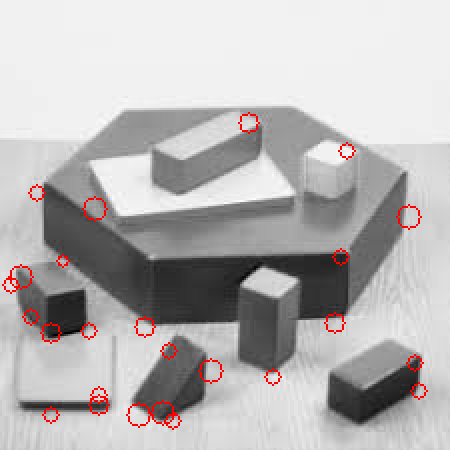
\includegraphics[width=0.4\textwidth]{figures/keypoints.png}
    \caption{Resultado esperado de la detección de puntos de interés y su orientación.}
    \label{fig:KPDet}
\end{figure}

Una vez obtenidas las imágenes gaussianas y los puntos de interés con sus orientaciones, se pueden generar los descriptores de las regiones vecinas a estos, que son invariantes a los cambios de iluminación y de punto de vista. En esta sesión se proporciona para ello la función \texttt{generateDescriptors()}.

\section*{Tarea C.6: Pipeline de generación de puntos clave y descriptores}
\phantomsection
\addcontentsline{toc}{section}{Tarea C.6: Pipeline de generación de puntos clave y descriptores}

En esta tarea deberá completar la función \texttt{computeKeypointsAndDescriptors()}. Esta función recibe la imagen original, el valor inicial de \textit{sigma} y el número de diferencias de gaussianas que se desea generar. Complétela con los métodos desarrollados en las tareas anteriores para obtener el \textit{pipeline} completo de localización de puntos de interés y generación de descriptores.

\section*{Tarea C.7: Correspondencia de características entre imágenes}
\phantomsection
\addcontentsline{toc}{section}{Tarea C.7: Correspondencia de características entre imágenes}

En esta tarea comprobará la capacidad del sistema para localizar las mismas características en una imagen alterada y establecer la correspondencia entre las características de la imagen original y las de la alterada. Para ello, cargue la imagen original y la alterada (\texttt{0.jpg} y \texttt{0\_rot.jpg}) en escala de grises con \texttt{cv2} y haga las llamadas pertinentes al método de la tarea anterior para obtener los puntos de interés y los descriptores de ambas imágenes.

Con estos datos, la función \texttt{matchFeatures\_and\_save()} establece la correspondencia entre los puntos de interés de ambas imágenes, la muestra y la guarda en la ruta indicada (por ejemplo, en \texttt{../results/partC/feature\_extraction/2\_match\_features}). Si solo quiere visualizarla, puede usar \texttt{matchFeatures()}. Ambas necesitan más de 10 correspondencias para dibujar el resultado. La Figura \ref{fig:FMatchEnd} muestra el resultado esperado.

\begin{figure}[h]
    \centering
    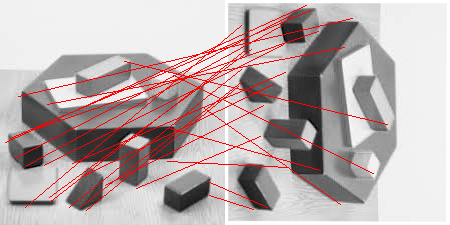
\includegraphics[width=0.8\textwidth]{figures/feature_match_mine.png}
    \caption{Resultado esperado de la correspondencia de características con el \textit{pipeline} desarrollado.}
    \label{fig:FMatchEnd}
\end{figure}

Una vez comprendido el funcionamiento de un detector de puntos de interés y de sus descriptores, se le anima a emplear el método propio de OpenCV, como se proporciona en el notebook (\textit{Ampliación: SIFT con OpenCV}).

\section*{Preguntas}
\addcontentsline{toc}{section}{Preguntas}

\vspace{5mm}
\begin{tcolorbox}[colback=gray!10, colframe=gray!30, coltitle=black, title=Pregunta C.1: Correspondencia de imágenes propias y evaluación, halign=left]
Con los métodos desarrollados para la extracción de características, use su \textit{pipeline} y el SIFT de OpenCV con sus propias imágenes (por ejemplo, dos fotos de un mismo objeto desde puntos de vista distintos). Adjunte los resultados de ambos y compárelos extrayendo sus propias conclusiones.
\end{tcolorbox}
